
\chapter{Data Classification}
\label{cha:data-classification}
First step towards this project is to fetch our data from Twitter. The data is classified into two
groups, relevant and irrelevant. We will be spending most of our time with the relevant data.

To carry out our experiments, we will need to filter out irrelevant tweets. Irrelevant tweets are
tweets which we do not really care about. Some examples include:

\begin{itemize}
  \item \textit{Every day I'm levelling! And now I'm level 19 in \#CSRClassics for iPhone!}
  \item \textit{Yes, our apple juice and cider are both GMO-free.}
  \item \textit{I just had my first carmel apple}
\end{itemize}

All three tweets could be regarded as relevant but for our use case, they are not. This is because
we are only interested in tweets that contain personal opinions about Apple Incorporated. Examples
of relevant tweets include: their thoughts
\begin{itemize}
  \item \textit{Once you get hooked to \#Mac, you will definitely go back to \#Windows! Lol!}
  \item \textit{If Tim Cook at Apple knows anything about him, it'd be to stay away from Icahn.}
\end{itemize}

Of course we can manually classify this data but when we have millions of tweets, this becomes
impracticable. This is where we employ some classification algorithms to assist us. This is a
three step process and we will discuss them in the next sub sections.

\section{Preparing train data}
\begin{figure}
  \begin{center}
    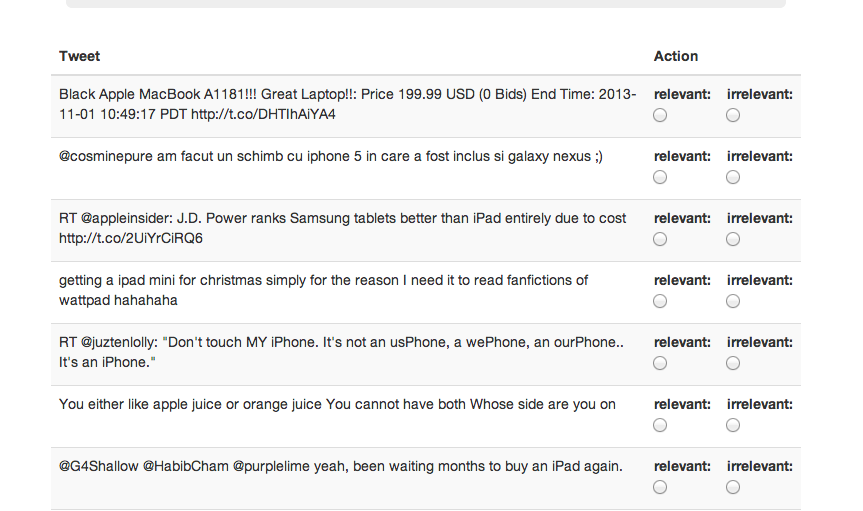
\includegraphics[scale=0.6]{Figures/datalabeller}
  \end{center}
  \caption{The data labelling application}
\label{fig:labeller}
\end{figure}

Train data, also known as a training set is a set of data used to train a knowledge database, in
this case, a classifier. Our training set will be created by manually labelling a fraction of our
dataset. People write in different ways on Twitter and trying to create a new training set to
encompass all possibilities would be very time consuming and intractable. To make this process a
little easier, a web application for labelling tweets was created. \Figref{fig:labeller} is a
screen shot of what the application looks like.

\begin{figure}
  \begin{center}
    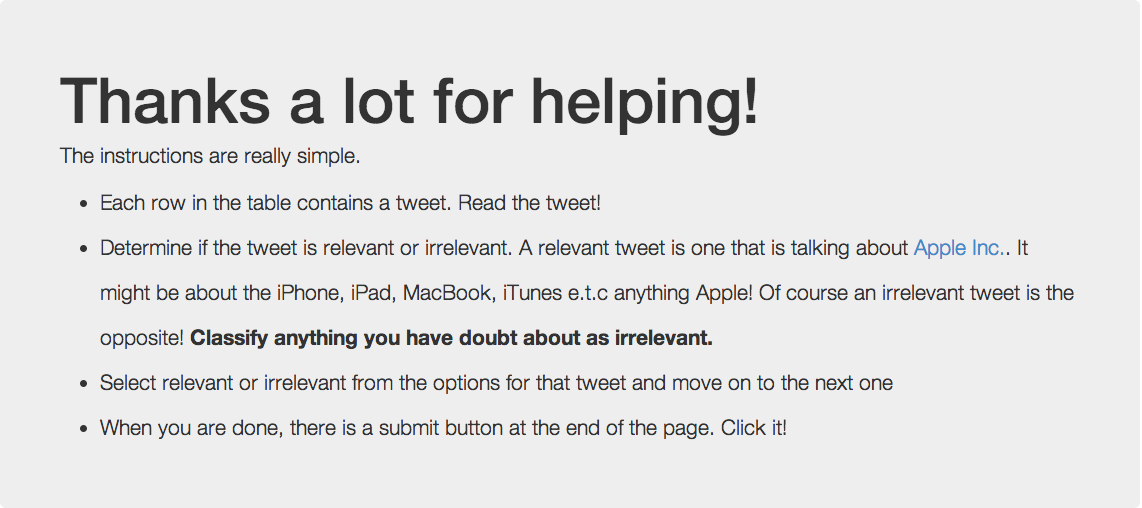
\includegraphics[scale=0.4]{Figures/labeller_instructions}
  \end{center}
  \caption{Instructions on how to label the tweets}
\label{fig:labeller-instructions}
\end{figure}

While using the web application in \Figref{fig:labeller} makes labelling tweets easier and a
little quicker, it does not change the fact the we still have to manually label a plethora of
tweets. To speed up this process even further, the data labeller was made public and the labelling
was crowd sourced. A list of instructions (\Figref{fig:labeller-instructions}) were also given
to anyone who helped label the tweets.

One problem with crowd sourcing this task is that people have different opinions about what is
relevant and what is not. In an attempt to solve this problem, each tweet was classified twice. A
tweet classified as relevant gets a score of 1 and an irrelevant tweet gets 0. This means that if a
tweet was classified twice as relevant, it should have a score of 2 and a tweet classified as
irrelevant twice should have a score of 0. Tweets that have been classified twice and have a total
score of 1 are tweets that have been classified as both relevant and irrelevant. These are tweets
that we have to classify ourselves into a group. While this is not an assured way of getting the
best training set, it gives us a certain level of confidence about our training set. It is also
arguably much better than single handedly creating the training set.

\section{Training a classifier}
\label{sec:training-classifier}
As discussed in Section~\ref{sec:bg-naive-bayes}, a Na\"{i}ve Bayes Classifier is a probabilistic
classifier which is based on the Bayes Theorem. We will train one and use it to classify the tweets
into relevant and irrelevant groups.

Unfortunately, the classifier takes as input a vector space representation of our tweets and not the
actual text. This means we have to convert our tweets into a vector representation of some sort. We
will be using the \textbf{bag of words model} in this study but before we transform the tweets, we
have to pre-process the tweets.

\subsection{Pre-processing}
\label{sec:classification-preprocessing}
Pre-processing are the tasks we have to carry out before the main transformation of the tweets to a
vector space model. Firstly, we will peruse through our tweets to remove new line characters, links
and stop words. We then take each tweet and convert it into a list of \textit{n-grams}.

Some tweets have special characters like new lines, excess spaces and Unicode characters and these
characters are irrelevant for our use-case. Every programming language has a function to strip
off newlines and whitespace and it can be easily done in one line of code. Removing the links from
the text is a little more complex and the ``easiest'' way to do this would be to use a regular
expression. \citet{friedl2006mastering} in his book \textit{Mastering Regular Expressions} describes
regular expressions as a very flexible mini language that is used for text processing. The regular
expression used can be found in Appendix~\ref{sec:appx-regular-expressions}.

Unfortunately, all a regular expression can do is search for patterns in text. Luckily, most
programming languages provide support for regular expressions so all we have to do is search for the
pattern in each tweet and use the language features to replace the matched pattern with nothing(an
empty string preferably).

The next step is to remove stop words in each tweet. \citet{wilbur1992automatic} defines a stop word
as ``\textit{a word which may be identified as a word that has the same likelihood of occurring in
those documents not relevant to a query as in those documents relevant to the query.}'' In other
words, stop words occur in every document irrespective of the document's relevance. Stop words are
usually the most common word in a language, English in this case. Some examples include
\textit{and}, \textit{or}, \textit{the} etc. Removal of stop words from text usually results in
better model performance as shown in \Figref{fig:auc-curves-stopwords} on page
\pageref{fig:auc-curves-stopwords}.

%TODO: reference a table in a future section that proves this.

Finally, we convert each tweet to a list of \textit{n-grams}. An n-gram ``\textit{is a contiguous
sequence of n items from a given sequence of text}''\footnote{See
http://en.wikipedia.org/wiki/N-gram}. The easiest way to understand n-grams is with an example.
Assuming we have a document with the text ``machine learning rocks''. All unigrams(n-grams
where n is 1) that can be extracted from that text are \textit{``machine''}, \textit{``learning''}
and \textit{``rocks''}. Also, all bigrams(n-grams where n is 2) in the document are
\textit{``machine learning''} and \textit{``learning rocks''}. In this study, we will be using a
combination of unigrams and bigrams.

We have discussed different preprocessing tasks that we have to apply to our documents before
transforming them into the bag of words matrix representation. In the next section, we will look
into how the bag of words model works and then transform our tweets into this model.


\subsection{Transforming tweets to bag-of-words}
The bag of words model is a common representation for text that involves representing a document as
a multiset of its words. It is a very common way to represent documents and it has also been used
recently in computer vision \citep{sivic2009efficient}. All sets are combined to form a
document-term matrix of the corpora. The rows represent each document while the columns represent
the occurrence/frequency of a word in that document. To show how this works, let us assume we have
the following documents:
\begin{description}
  \item[A] today is a sunny day.
  \item[B] it is a sunny day isn't it?
  \item[C] what a sunny day!
\end{description}

% TODO: add isn't to table
\begin{table}
  \begin{center}
    \begin{tabular}{|c|c c c c c c c|}
      \hline
      & today & what & it & is & a & sunny & day \\
      \hline
      A & 1 & 0 & 0 & 1 & 1 & 1 & 1 \\
      B & 0 & 0 & 2 & 1 & 1 & 1 & 1 \\
      C & 0 & 1 & 0 & 0 & 1 & 1 & 1 \\
      \hline
    \end{tabular}
    \caption{A bag-of-words representation}
    \label{tab:document-term-matrix}
  \end{center}
\end{table}

By the above definition, \Tableref{tab:document-term-matrix} will be an accurate representation
of our sentences using the bag of words model. Note that in our example, each sentence is a document
and all sentences form the corpora.

Now that we have converted our corpora into a bag of words representation, we will now use the
resulting matrix to train our classifier.

\subsection{Training the initial classifier}

\begin{table}
  \begin{subtable}{.5\linewidth}
    \centering
    \begin{tabular}{cccc} \toprule
      accuracy        & std($\sigma$) & AUC             & std($\sigma$) \\ \midrule
      0.9875          & 0.0000        & 0.7387          & 0.0000 \\
      0.9877          & 0.0002        & 0.7381          & 0.0000 \\
      \textbf{0.9878} & 0.0002        & 0.7312          & 0.0090 \\
      0.9877          & 0.0002        & 0.7412          & 0.0190 \\
      \textbf{0.9878} & 0.0002        & 0.7454          & 0.0190 \\ \midrule
      0.9876          & 0.0005        & 0.7394          & 0.0220 \\
      0.9875          & 0.0005        & 0.7431          & 0.0220 \\
      0.9874          & 0.0005        & 0.7427          & 0.0200 \\
      0.9874          & 0.0005        & \textbf{0.7455} & 0.0210 \\
      0.9873          & 0.0005        & 0.7454          & 0.0200 \\ \bottomrule
    \end{tabular}
      \caption{With stop words}
      \label{tab:data-with-stopwords}
  \end{subtable}
  % =======================
  \begin{subtable}{.5\linewidth}
    \centering
    \begin{tabular}{cccc} \toprule
      accuracy        & std($\sigma$) & AUC             & std($\sigma$) \\ \midrule
      \textbf{0.9908} & 0.0000        & 0.7526          & 0.0000 \\
      0.9904          & 0.0004        & 0.7589          & 0.0060 \\
      0.9903          & 0.0003        & 0.7485          & 0.0150 \\
      0.9901          & 0.0004        & 0.7535          & 0.0160 \\
      0.9901          & 0.0003        & 0.7572          & 0.0160 \\ \midrule
      0.9901          & 0.0003        & 0.7582          & 0.0150 \\
      0.9902          & 0.0004        & \textbf{0.7618} & 0.0160 \\
      0.9901          & 0.0004        & 0.7587          & 0.0170 \\
      0.9901          & 0.0004        & 0.7592          & 0.0160 \\
      0.9900          & 0.0004        & 0.7572          & 0.0160 \\ \bottomrule
    \end{tabular}
      \caption{Without stop words}
      \label{tab:data-without-stopwords}
  \end{subtable}
\caption{Accuracy and AUC for 10-fold cross validation}
\label{tab:with-without-stopwords-data-tables}
\end{table}

In \Sectionref{sec:classification-preprocessing}, we looked at different pre-processing tasks to be
carried out, one of which was the removal of stop words. In this section, we train two classifiers,
one with stop words in our data and the other with stop words removed from the data. We then three
different but complementary methods. They include:

\begin{description}
  \item[Accuracy:] This is the degree to which our classifier is correct. For instance, if we give
    it 20 instances and it rightly classifies 7, then we say our classifier is 70\% accurate. The
    problem with accuracy is that the value does not take into consideration the number of false
    positives or false negatives. So for instances, how many relevant samples were classified as
    irrelevant and vice versa. Research  by \citet{ling2003auc} shows that accuracy is also not a
    good measure when dealing with unbalanced classes. Our dataset is highly unbalanced so we cannot
    use accuracy to evaluate performance.

  \item[Receiver Operating Characteristic curve:] The ROC curve was introduced in signal processing
    and used to evaluate the prediction power of different classification algorithms. More
    importantly, the area under this curve, referrred to henceforth as AUC, is the metric used to
    compare the performance of different classifiers \citep{bradley1997use}. As \citet{ling2003auc,
    huang2005using} describes, AUC is generally a better measure because it takes into consideration
    the precision an sensitivity(also called recall) of the classifier\footnote{See
      \url{http://en.wikipedia.org/wiki/Precision_and_recall} for a more detailed explanation of
    precision and recall}. The ROC curve is created by plotting the precision of a classifier
    against its sensitivity.

  \item[K-fold Cross Validation:] Training and validating/testing a classifier with the same dataset
    is ineffective because the classifier simply labels examples it has just seen. This problem is
    called overfitting and to solve it, we use the k-fold cross validation technique. The idea is to
    split our data into $k$ folds\footnote{A fold is essentially a fraction of the dataset}, train
    the classifier on $k-1$ folds and test on the remaining fold. This process is repeated $k$ times
    to ensure every fold has been used for validation.
\end{description}

Tables~\ref{tab:data-with-stopwords} and~\ref{tab:data-without-stopwords} contains a list of values
representing the result of running 10-fold cross validation on our trained classifier with and
without stop words, respectively. It also depicts the accuracy, AUC and standard deviation between
folds but we shall focus more on the AUC.

We can see from the tables that the standard deviation($\sigma$) is very low. A low standard
deviation indicates that there is not much variation between folds and the values are very close to
the mean value. Comparing the highest AUC in both tables(values in bold), we can see that the
removal of stop words gives us approximately 2.2\%(from 0.7455 to 0.7618 AUC) increase in AUC\@.
Figures~\ref{fig:auc-with-stopwords} and~\ref{fig:auc-without-stopwords} gives a visual
representation of the AUC curve. The value used in the plots is the average AUC over all folds.
This increase proves that training a classifier without stop words in our dataset gives better
performance.

While 0.76 is an acceptable AUC, it turns out we can do even better and the next section shows how
we can achieve this.

\begin{figure}
  \centering
  \begin{subfigure}[b]{0.49\linewidth}
    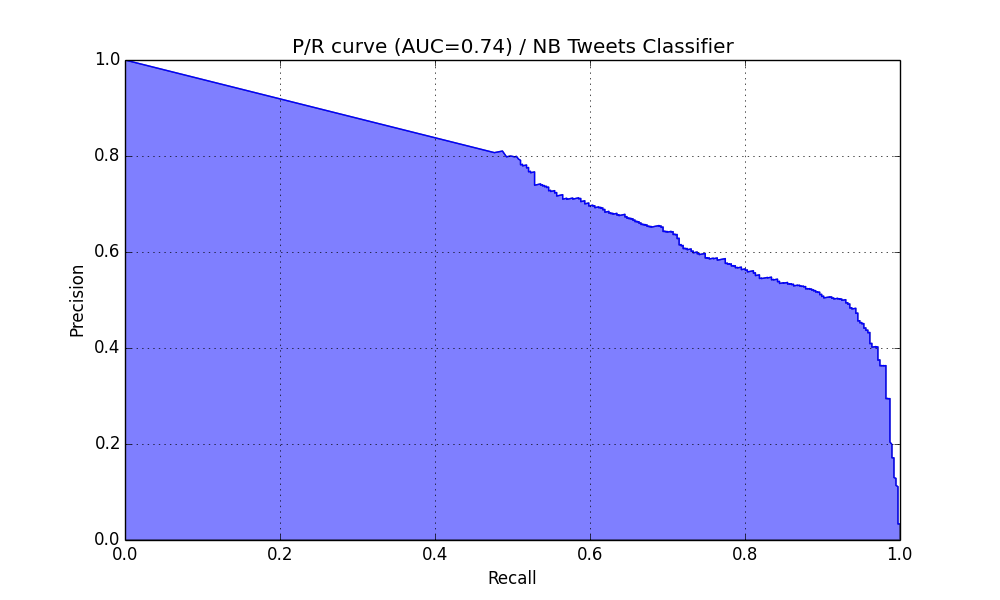
\includegraphics[width=\linewidth]{Figures/pr_NB_Tweets_Classifier_01}
  \caption{AUC=74 with stop words}
  \label{fig:auc-with-stopwords}
  \end{subfigure}
  % =============
  \begin{subfigure}[b]{0.49\linewidth}
      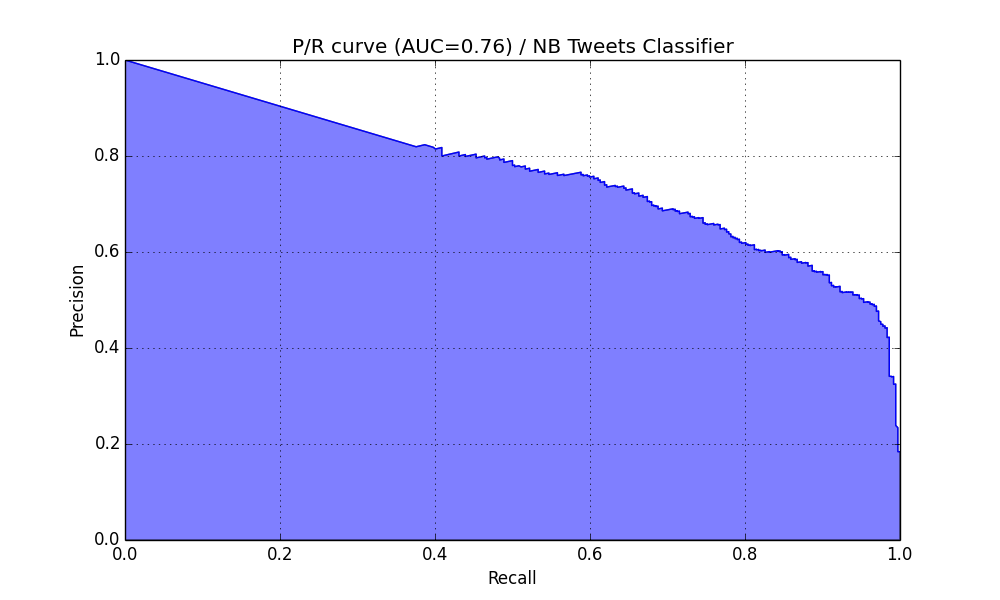
\includegraphics[width=\linewidth]{Figures/pr_NB_Tweets_Classifier_02}
  \caption{AUC=76 without stop words}
  \label{fig:auc-without-stopwords}
  \end{subfigure}
\caption{AUC curves with and without stop words}
\label{fig:auc-curves-stopwords}
\end{figure}



\subsection{Improving the classifier}

\begin{table}
  \centering
  \begin{tabular}{cccc} \toprule
    accuracy        & std($\sigma$) & AUC             & std($\sigma$) \\ \midrule
    0.9939          & 0.0000        & \textbf{0.8068} & 0.0000 \\
    0.9939          & 0.0000        & 0.8006          & 0.0062 \\
    \textbf{0.9949} & 0.0001        & 0.7893          & 0.0167 \\
    0.9939          & 0.0003        & 0.7960          & 0.0186 \\
    0.9939          & 0.0003        & 0.7892          & 0.0215 \\ \midrule
    0.9939          & 0.0004        & 0.7920          & 0.0206 \\
    0.9939          & 0.0004        & 0.7902          & 0.0196 \\
    0.9939          & 0.0004        & 0.7900          & 0.0183 \\
    0.9939          & 0.0004        & 0.7890          & 0.0175 \\
    0.9939          & 0.0004        & 0.7876          & 0.0171 \\ \bottomrule
  \end{tabular}
    \caption{Accuracy and AUC for tfidf weighted model}
    \label{tab:tfidf-model-table}
\end{table}

In the previous section we were able to get up to 0.76 AUC\@. In this section we explore two ways of
improving this value. Firstly, we look into a new type of vector space model for representing our
corpus called the tf-idf weighting scheme. We briefly look at how it is different from the bag of
words model and what makes it better. Secondly, we try to train multiple classifiers with
different combinations of model parameters to try to find the best possible match of parameters.


\subsubsection{Using TF-IDF Weighting Scheme}
TF-IDF stands for Term Frequency-Inverse Document Frequency is a weighting scheme that can be used
to determine the importance of a word to a document in a corpus. Up until now, we have been using
the bag-of-words representation which gives us the term\footnote{A term is also a word in this case}
frequency. However, this is inadequate because a document with 5 occurrences of a word is not
necessarily 5 times relevant than a document with only 1 occurrence of the same word. This is where
the inverse document frequency comes in.

The inverse document frequency measures how important a word is in a document. It weighs down terms
with a high frequency while weighing up the terms with lower occurrences. This is useful mainly
because we can get rid of stop words that do not appear in our stop words list.

\Tableref{tab:tfidf-model-table} shows use the results of running 10-fold cross validation using the
tf-idf scheme. We can see that our standard deviation remains low, as in the previous section which
is good but more importantly, we have a tremendous increase in AUC\@. We achieved approximately
0.76 AUC in the previous section and our highest value after using the tf-idf weighting scheme is
approximately 0.80 AUC which is a 5.7\% increase in AUC\@. \Figref{fig:auc-tfidf} is a visual
representation of the area under the ROC curve, AUC\@. The value used in the plot is the average AUC
over all folds.

\begin{figure}
  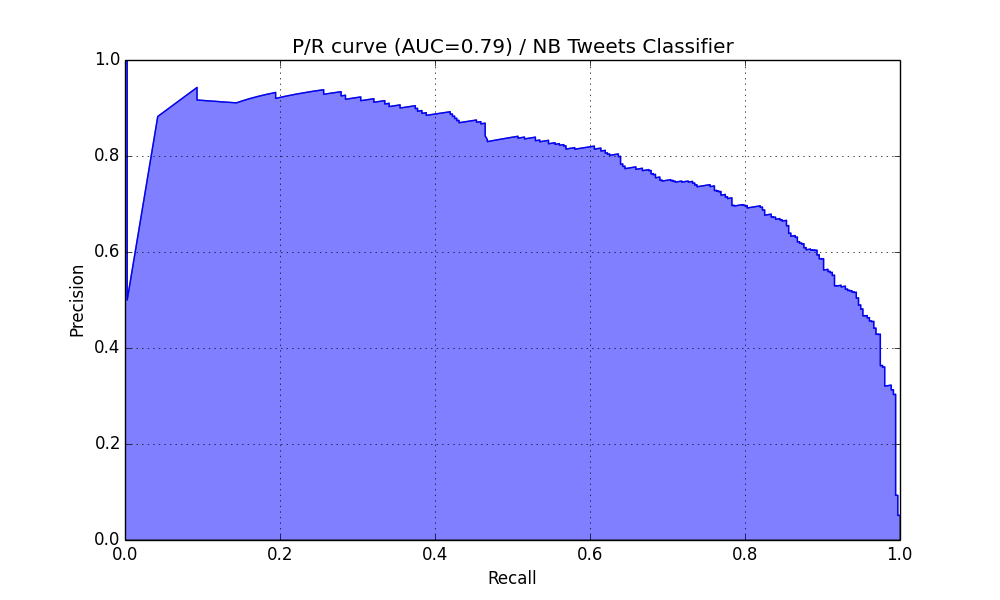
\includegraphics[width=\linewidth]{Figures/pr_NB_Tweets_Classifier_03}
\caption{AUC curve for tf-idf weighted corpora}
\label{fig:auc-tfidf}
\end{figure}



\subsubsection{Exhaustive Grid Search}
\label{sec:exhaustive-grid-search}

% \begin{table}
%   \centering
%   \begin{tabular}{cccc} \toprule
%     accuracy        & std($\sigma$) & AUC             & std($\sigma$) \\ \midrule
%     \textbf{0.9961} & 0.0000        & 0.8415          & 0.0000 \\
%     0.9960          & 0.0001        & \textbf{0.8610} & 0.0195 \\
%     0.9955          & 0.0007        & 0.8445          & 0.0282 \\
%     0.9955          & 0.0006        & 0.8491          & 0.0257 \\
%     0.9954          & 0.0005        & 0.8441          & 0.0251 \\ \midrule
%     0.9954          & 0.0005        & 0.8447          & 0.0229 \\
%     0.9954          & 0.0005        & 0.8465          & 0.0217 \\
%     0.9954          & 0.0004        & 0.8470          & 0.0203 \\
%     0.9954          & 0.0004        & 0.8468          & 0.0192 \\
%     0.9954          & 0.0004        & 0.8487          & 0.0191 \\ \bottomrule
%   \end{tabular}
%     \caption{Accuracy and AUC for best model}
%     \label{tab:best-model}
% \end{table}



% \begin{figure}
%   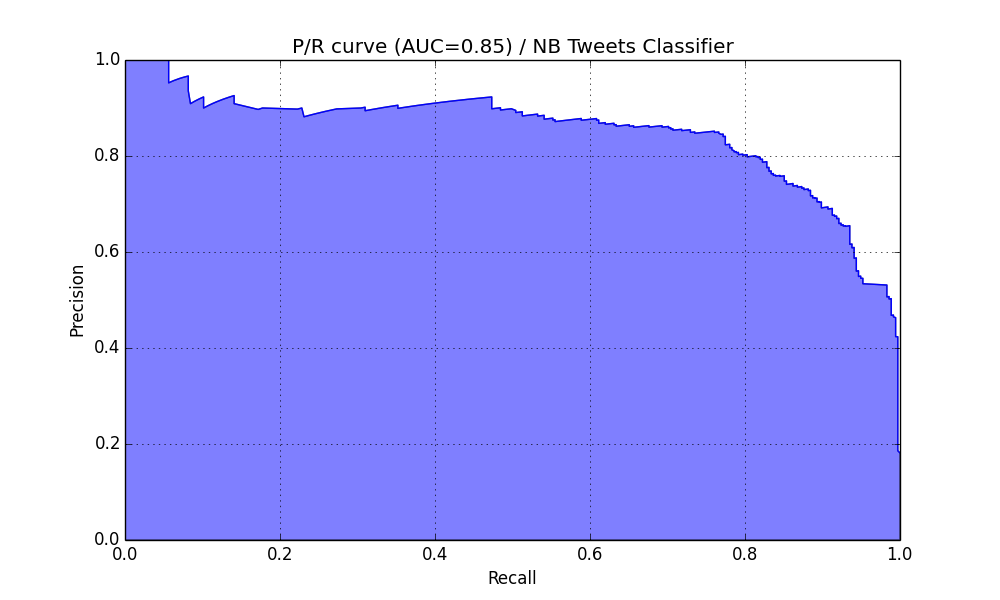
\includegraphics[width=\linewidth]{Figures/pr_NB_Tweets_Classifier_04}
% \caption{AUC curve for best found model}
% \label{fig:auc-best-model}
% \end{figure}

